% !TeX root = main.tex

\chapter{Real time reccurent learning}

A partir de cette section, les objectifs sont de reconnaître une chaine de
caractère en temps réel : c'est à dire que en donnant un ou plusieurs caractères
, on doit être capable de prédire la fin de la chaine. Ce genre de problème peut
 être étendu à la recherche comportementale en temps réel. Pour résoudre ce
genre de problème, on utilise des réseaux neuronaux récurrents, qui ont
l'avantage de se souvenir des états précedents pour pouvoir prédire efficacement
 les états suivants; ils comportent une mémoire courte. Dans un premier temps,
nous allons nous interesser aux réseaux RTRL.

\section{Théorie}

Dans la suite, nous allons nous interesser au problème de la grammaire de Reber,
 qui servira d'échantillon de test pour RTRL.

\subsection{La grammaire de Reber}

 Une grammaire de Reber est un langage défini par l'automate déterministe
 cyclique suivant :

\begin{figure}[!ht]
\begin{center}
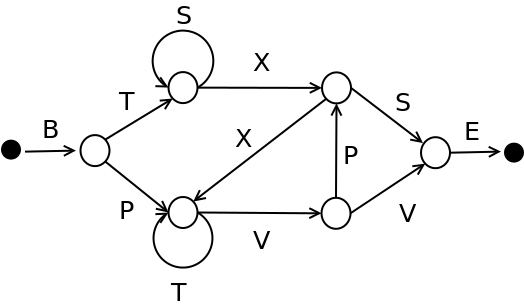
\includegraphics[scale=0.4]{rtrl/reberGrammar.png}
\end{center}
\caption{Grammaire de Reber simple}
\end{figure}


De base, on considère une probabilité uniforme de chosir l'état suivant parmis
les états possibles suivants. La lettre $B$ et la lettre $E$ sont des lettres
indiquant simplement le début et la fin de la chaîne, elles n'ont pas d'interet
propre pour la grammaire. Les autres lettres présentes sur les arêtes peuvent
variées, mais elles doivent respecter les règles suivantes :
\medskip
\begin{itemize}
	\item Chaque lettre doit apparaitre exactement deux fois
	\item On ne peut pas obtenir deux lettres consécutives en passant par des états différents.
\end{itemize}

\vspace{\parskip}
L'interet de la grammaire de Reber est que c'est un automate simple qui ne nécessite que la mémoire de la dernière et de l'avant dernière lettre pour trouver la suivante. En effet, d'après la dernière règle, connaitre les deux dernières lettres impose l'état actuel dans l'automate. En outre, chaque lettre apparaissant deux fois, la connaissance seule de la dernière lettre ne suffit pas à prédir la suivante correctement. On remarque que l'on peut résoudre ce problème avec un perceptron classique si on donne en entrée du perceptron les deux dernières lettres du mot. Ce modèle bien que résolvant ce problème, n'est pas adapté au calcul en temps réel. De plus il ne résout pas le problème de la grammaire de Reber double.

Le problème de la grammaire double est un problème similaire à la grmmaire simple. L'automate le représentant est :

\begin{figure}[!ht]
\begin{center}
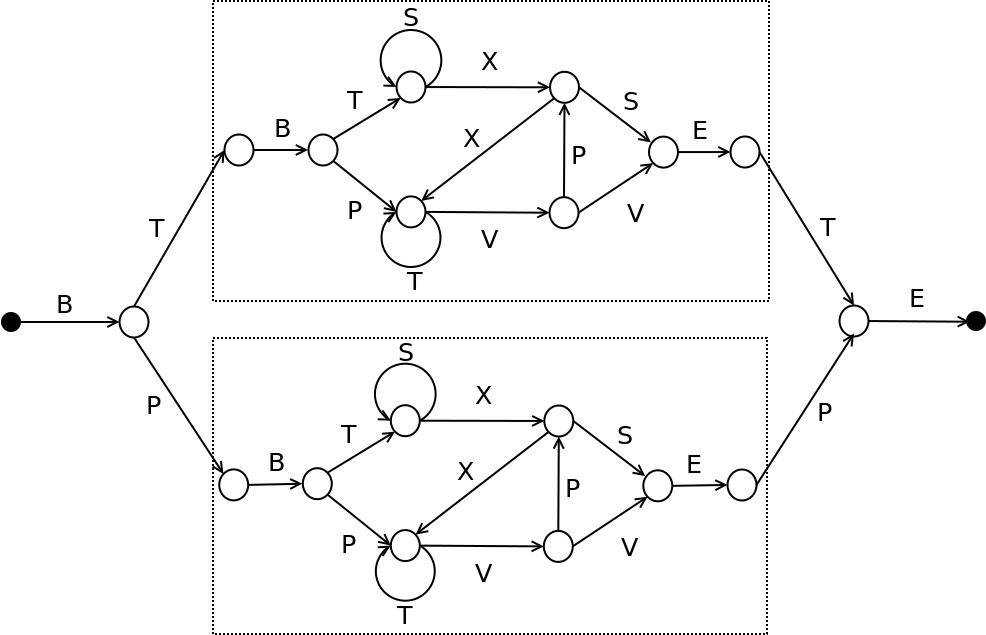
\includegraphics[scale=0.4]{rtrl/reberGrammarSymmetric.png}
\end{center}
\caption{Grammaire de Reber symetrique}
\end{figure}

On remarque qu'il est consitué de deux grammaires de Reber simple qui sont reliés en entrée et en sortie. La difficulté de ce problème est qu'il faut mémorisé la première valeur pour en déduire la dernière. Dans ce cas, une mémoire ''infini'' est nécessaire theoriquement pour se souvenir de la première entrée. Il est donc impensable d'utiliser de la même façon un réseau de perceptron classique. On a alors besoin de réseau récurrent, dont la sortie à un instant $t$ va dépendre de la sortie à un instant $t-1$.

\subsection{Réseau RTRL}
